%%% License: Creative Commons Attribution Share Alike 4.0 (see https://creativecommons.org/licenses/by-sa/4.0/)

\documentclass[english,10pt
,aspectratio=169
%,handout
%%%%%,notes
]{beamer}
%%% License: Creative Commons Attribution Share Alike 4.0 (see https://creativecommons.org/licenses/by-sa/4.0/)

\DeclareGraphicsExtensions{.eps, .pdf,.png,.jpg,.mps,}
\usetheme{reMedian}
\usepackage{parskip}
\makeatother

\renewcommand{\baselinestretch}{1.1} 

\usepackage{amsmath, amssymb, amsfonts, amsthm}
\usepackage{enumerate}
%\usepackage{enumitem}
\usepackage{hyperref}
\usepackage{url}
\usepackage{bbm}
\usepackage{color}

\usepackage{tikz}
\usepackage{tikzscale}
\newcommand*\circled[1]{\tikz[baseline=(char.base)]{
		\node[shape=circle,draw, inner sep=-20pt] (char) {#1};}}
\usetikzlibrary{automata,positioning}
\usetikzlibrary{decorations.pathreplacing}
\usepackage{pgfplots}
\usepgfplotslibrary{fillbetween}
\usepackage{graphicx}

\usepackage{setspace}
\thinmuskip=1mu
\medmuskip=1mu 
\thickmuskip=1mu 


\usecolortheme{default}
\usepackage{verbatim}
\usepackage[normalem]{ulem}

\usepackage{apptools}
\AtAppendix{
	\setbeamertemplate{frame numbering}[none]
}
\usepackage{natbib}


% red strikeout
\newcommand\soutred{\bgroup\markoverwith
	{\textcolor{red}{\rule[0.55ex]{2pt}{0.8pt}}}\ULon}



% To use LyX frames from old version:
\def\lyxframeend{} % In case there is a superfluous frame end
\long\def\lyxframe#1{\@lyxframe#1\@lyxframestop}%
\def\@lyxframe{\@ifnextchar<{\@@lyxframe}{\@@lyxframe<*>}}%
\def\@@lyxframe<#1>{\@ifnextchar[{\@@@lyxframe<#1>}{\@@@lyxframe<#1>[]}}
\def\@@@lyxframe<#1>[{\@ifnextchar<{\@@@@@lyxframe<#1>[}{\@@@@lyxframe<#1>[<*>][}}
\def\@@@@@lyxframe<#1>[#2]{\@ifnextchar[{\@@@@lyxframe<#1>[#2]}{\@@@@lyxframe<#1>[#2][]}}
\long\def\@@@@lyxframe<#1>[#2][#3]#4\@lyxframestop#5\lyxframeend{%
	\frame<#1>[#2][#3]{\frametitle{#4}#5}}


\title{Mechanism Design}

\subtitle{1: Efficient Mechanisms}

\author{Egor Starkov}

\date{K{\o}benhavns Unversitet \\
	Fall 2021}


\begin{document}
	\AtBeginSection[]{
		\frame{
			\frametitle{This slide deck:}
			\tableofcontents[currentsection,currentsubsection]
	}}
	\frame[plain]{\titlepage}

\note{
	\begin{itemize}
		\item Last time we talked about seemingly nothing at all. Some concepts, some logistics, some introductions and technical difficulties -- and we finished early.
		\item We actually covered some core ideas and concepts. Today we will define those concepts formally.
		\item It will seem like repetition. But it's not.
		When you want to draw a plot in mathematica -- you know that `x' is a variable that should be on horizontal axis. But the computer does not. You need to put a line of code saying ``x is a variable''. Math is like computer. To use all the cool stuff from future lectures we need to introduce all the formal mathematical objects that it can work with. Today we'll do that.
		\item %2020 only
		Question last time: what's the line between CT and MD? MD is focused on shaping \emph{interactions} between many agents.
	\end{itemize}
}



%\begin{frame}
%	(math exercise from notes)
%\end{frame}
%\note{
%	\begin{itemize}
%		\item asked to read mathreview -- how many did that?
%		\begin{itemize}
%			\item introduce quick survey protocol (1s in chat)
%		\end{itemize}
%		\item $\int_a^b x^2 \log (x) dx$: $u=\log(x)$, $dv = x^2 dx$, so $du = 1/x dx$, $v = \frac{x^3}{3}$ and
%		\begin{align*}
%			\int_a^b x^2 \log (x) dx 
%			&= \left(\frac{x^3}{3}\log(x) \right)|_a^b - \int_a^b \frac{x^2}{3} dx
%			\\
%			&= \left(\frac{x^3}{3}\log(x) - \frac{x^3}{9} \right)|_a^b
%		\end{align*}
%	\end{itemize}
%}


\section{Defining a Mechanism}

\begin{frame}{What is a mechanism?}
	Let's reverse engineer from a simpler question:
	\textbf{What is a game?}
	\begin{enumerate}
		\item Set of players $i \in\{ 1,...,N\}$
		\item Set of actions $A_i$ for every $i$; set of action profiles $A \equiv \times_{i \in N} A_i$
		\item Collection of utility functions $u_i: A \to \mathbb{R}$
	\end{enumerate}
	(This is a \emph{normal-form game}. All extensive-form games (``trees'') and incomplete-information games can be represented as normal-form games.)
	
	Which parts of this definition are fixed at a higher level, and which can we \emph{design} as a part of a \emph{mechanism}?
\end{frame}


\begin{frame}{Problem environment}
	\centering
	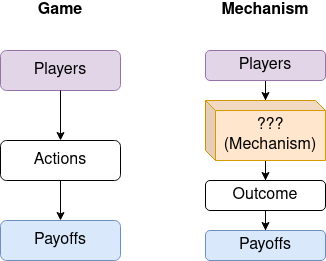
\includegraphics[scale=0.7]{pics/M1/game_vs_mech}
\end{frame}


\begin{frame}{General Problem Set-up}
	In our MD problem, the following environment will be \textbf{fixed}:
	\begin{itemize}
		\item $N$ agents,
		\item set $X$ of \alert{outcomes},
		\item each agent $i$ has \alert{type} $\theta_i\in\Theta_{i}$:
		\begin{itemize}
			\item describes agent's \structure{information},
			\item describes agent's \structure{preferences};
		\end{itemize}
		\item the type profile $\theta=(\theta_1,\dots,\theta_{N})$ is distributed according to a distribution $F$ with p.d.f. $\phi$,
		\begin{itemize}
			\item (often a missing subscript denotes a vector of respective objects)
			\item distribution $F$ is commonly known and agreed upon
		\end{itemize}
		\item each agent has a \alert{utility} function $u_{i}(x,\theta_{i})$ that depends on the collective choice $x \in X$ and his type $\theta_i$,
	\end{itemize}
\end{frame}


\begin{frame}{Social Choice Function}
	\begin{definition}[Social choice function]
		A \alert{social choice function} is a function \alert{$f:\Theta_{1}\times \dots\times\Theta_{N}\rightarrow X$} that assigns to each profile of types $(\theta_{1},\dots,\theta_{N})$ a collective choice $f(\theta_{1},\dots,\theta_{N})\in X$.
	\end{definition}
	\begin{itemize}
		\item gives a desired outcome as a function of the agents' types
	\end{itemize}
\end{frame}


\begin{frame}{Mechanism}
	\begin{itemize}
		\item a mechanism is a game played by the agents
		\item each agent has an action set $A_{i}$ in this game
	\end{itemize}
	\begin{definition}[mechanism]
		A \alert{mechanism} $\Gamma=(A_{1},\dots,A_{N},g(\cdot))$ is a collection of: 
		\begin{itemize}
			\item N \structure{strategy sets} $(A_{1},\dots,A_{N})$ and 
			\item an \structure{outcome function} $g:A_{1}\times\dots\times A_{N}\rightarrow X$.
		\end{itemize}
	\end{definition}
\end{frame}


\begin{frame}{Implementation}
	\begin{definition}[implementation]
		Mechanism $\alert{\Gamma}=(A_{1},\dots,A_{N},g(\cdot))$ \alert{implements} the s.c.f. $\alert{f}$ if there is \structure{an equilibrium} strategy profile $(a_{1}^{*},\dots,a_{N}^{*})$ of the Bayesian game induced by $\Gamma$ \structure{such that} 
		$$\structure{g}(a_{1}^{*}(\theta_{1}),\dots,a_{N}^{*}(\theta_{N})) = \structure{f} (\theta_{1},\dots,\theta_{N})$$ 
		for all $(\theta_{1},\dots,\theta_{N})\in\Theta_{1}\times\dots \times\Theta_{N}$.
	\end{definition}
\end{frame}


\begin{frame}{Summary of definitions}
	\begin{itemize}
		\item S.c.f. $f$ describes what we want to achieve;
		\item Mechanism $\Gamma = (S,g)$ describes what we do and how;
		\item Implementability says whether we have achieved our goal.
	\end{itemize}
\end{frame}


\begin{frame}{Full problem setup}
	\centering
	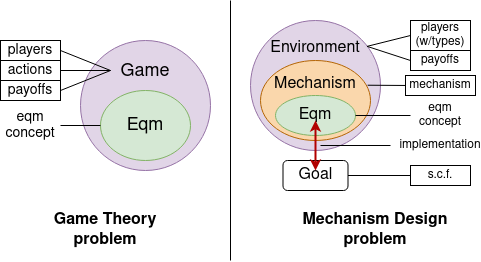
\includegraphics[scale=0.7]{pics/M1/game_vs_mech2}
\end{frame}


%\begin{frame}
%	(mechanism proposals)
%\end{frame}



\section{Revelation Principle}

\begin{frame}{Revelation Principle}
	\begin{itemize}
		\item Main cheat in Mechanism Design! No need to bruteforce through uncountable numbers of different games! It is enough to just... \only<1>{(\href{https://www.youtube.com/watch?v=dQw4w9WgXcQ}{{click to see more}})}
		\pause
		\item Instead of making players play the game, ask them for their $\theta_i$ and promise to play on their behalf!
		\item Requires that the designer has commitment power.
		\begin{itemize}
			\item Strong assumption, sometimes reasonable(?)
			\item The necessary evil for our purposes.
		\end{itemize}
	\end{itemize}
\end{frame}


\begin{frame}{Revelation Principle: Definitions}
	Fix some s.c.f. $f:\Theta \to X$.
	\begin{definition}[Direct revelation mechanism]
		A \structure{direct revelation mechanism} for $f$ is a mechanism in which $A_i = \Theta_i$ for all $i$ and $g(\theta) = f(\theta)$
	\end{definition}
	
	\begin{definition}[Truthuful implementation]
		S.c.f. $f$ is \structure{truthfully implementable} if it can be implemented by a direct revelation mechanism.
	\end{definition}
\end{frame}


\begin{frame}{Revelation Principle: Statement}
	\begin{block}{Revelation principle (blanket statement)}
		Suppose there exists a mechanism $\Gamma=(A_{1},\dots,A_{N},g)$ that implements the social choice function $f$.\\ Then $f$ is \structure{truthfully implementable}.
	\end{block}
	\medskip
	\begin{itemize}
		\item The statement above is informal.
		\begin{itemize}
			\item ``Implementation'' requires ``an equilibrium'', which can mean a million different things.
		\end{itemize}
		\item We will now focus on specific equilibrium concepts.
	\end{itemize}
\end{frame}
\note{
	\begin{itemize}
		\item We cannot fool agents by designing a very complicated game -- because they are rational and will compute the optimal strategy regardless
		\begin{itemize}
			\item This is, in part, to impose discipline our models -- if can deceive or confuse players then why not just do that.
			\item Economics is the science about being ``technically truthfull'' -- can never lie in equilibrium.
		\end{itemize}
		\item We need a formal equilibrium concept, so let's introduce one...
		\begin{itemize}
			\item Who knows which eqm concepts?
		\end{itemize}
	\end{itemize}
}




\section{Dominant Strategy Implementation}

%TODO 2020: switch from s and S to a and A since there are all actions, not strategies.
%TODO2021: was that the right call?
\begin{frame}{Recap: Dominant Strategy}
	\begin{itemize}
		\item strategy $a_i$ is a full contingent plan of play
		\item strategy $a_i$ is \alert{dominant} for agent $i$ if it is best \emph{no matter what the other players do}
	\end{itemize}
	\begin{definition}[dominant strategy]
		Given mechanism $\Gamma=(A,g)$,
		$a_{i}: \Theta_{i}\rightarrow A_{i}$ is a \structure{dominant strategy} if for all $\theta_{i}\in \Theta_{i}$
		$$ u_{i}(g(a_{i}(\theta_{i}),a_{-i}),\theta_{i})\geq u_{i}(g(\hat a_{i},a_{-i}),\theta_{i})$$
		for all $\hat a_{i}\in A_{i}$  and all $a_{-i}\in A_{-i}$.
	\end{definition}
	\begin{itemize}
		\item our definition slightly different from the standard -- does not require strict inequality
	\end{itemize}
\end{frame}


\begin{frame}{Dominant Strategy Equilibrium}
	\begin{itemize}
		\item in a \alert{dominant strategy equilibrium} every player plays a dominant strategy
	\end{itemize}
	\begin{definition}[dominant strategy equilibrium]
		A strategy profile $(a_1^*,\dots,a_N^*)$ is a \structure{dominant strategy equilibrium} of mechanism  $\Gamma=(A_{1},\dots,A_{N},g)$ if for all $i$ and all $\theta_{i}\in \Theta_{i}$
		$$ u_{i}(g(a_{i}^{*}(\theta_{i}),a_{-i}),\theta_{i}) \geq u_{i}(g(\hat a_{i},a_{-i}), \theta_{i})$$
		for all $\hat a_{i}\in A_{i}$ and all $a_{-i}\in A_{-i}$.
	\end{definition}

	Now let's finally be formal about all our definitions.
\end{frame}


\begin{frame}{Dominant Strategy Implementation}
	\begin{itemize}
		\item A mechanism \alert{implements $f$ in dominant strategies} if
		\begin{itemize}
			\item the game induced by the mechanism has a dominant strategy equilibrium
			\item the outcome in this equilibrium coincides with $f$
		\end{itemize}
	\end{itemize}
	\begin{definition}[implementation in dominant strategies]
		A mechanism $\Gamma=(A_{1},\dots,A_{N},g)$ \structure{implements} the social choice function $f$ \structure{in dominant strategies} if there exists a dominant strategy equilibrium $(a_1^*,\dots,a_N^*)$ of $\Gamma$ such that $g(a_1^*(\theta_{1}),\dots,a_N^*(\theta_{N}))=f(\theta)$ for all $\theta\in\Theta$.
	\end{definition}
\end{frame}


\begin{frame}{Good Implementation Concept?}
	\begin{itemize}
		\item very robust equilibrium concept
		\begin{itemize}
			\item no need to predict what the other players will play
			\item no need to know the type distribution $\phi$
			\item works even if
			\begin{itemize}
				\item players don't know $\phi$ or even if players believe in different $\phi_{i}$ (protects from players' model misspecification)
				\item players think that other players are not rational
			\end{itemize}
		\end{itemize}
		\item not a panacea
		\begin{itemize}
			\item does not rule out other weird Nash Equilibria (remember SPA)
			\item is not necessarily collusion-proof
			\item does not protect from designer's model misspecification
		\end{itemize}
	\end{itemize}
	Bottom line: it's as good as they get, but far from perfect.
\end{frame}


\begin{frame}{Dominant Strategy Incentive Compatibility}
	\begin{theorem}[Revelation Principle for Dominant Strategies]
		Suppose there exists a mechanism $\Gamma=(A_{1},\dots,A_{N},g)$ that implements the social choice function $f$ in dominant strategies.\\ Then $f$ is \structure{truthfully implementable} in dominant strategies.
	\end{theorem}
	\medskip
	\begin{definition}[Dominant Strategy Incentive Compatibility]
		``$f$ is \alert{dominant strategy incentive compatible} (DSIC)''\\ 
		means the exact same thing as \\
		``$f$ is \structure{truthfully implementable in dominant strategies}''.
	\end{definition}
\end{frame}


\begin{frame}{DS Revelation Principle: Proof}
	Let $\Gamma$ implement $f$ in dominant strategies, i.e. there is a strategy profile  $(a_1^*,\dots,a_N^*)$ such that $g(a_1^*(\theta_{1}),\dots,a_N^*(\theta_{N}))=f(\theta)$ for all $\theta$, and for all $i$ and  $\theta_{i}\in\Theta_{i}$,
	$$ u_{i}(g(a_{i}^{*}(\theta_{i}),a_{-i}),\theta_{i})\geq u_{i}(g(\hat a_{i},a_{-i}),\theta_{i})$$
	for all $\hat a_{i}\in A_{i}$ and all $a_{-i}\in A_{-i}$. 
	
	Then
	$$ u_{i}(g(a_{i}^{*}(\theta_{i}), a_{-i}^{*}(\theta_{-i})),\theta_{i})\geq u_i (g(a^*_i(\hat{\theta}_i), a_{-i}^{*}(\theta_{-i})), \theta_i)$$
	for all $\hat{\theta}_i \in \Theta_i$, $\theta_{-i} \in \Theta_{-i}$. 
	
	Since $g(a^*(\theta)) = f(\theta)$,
	$$ u_i (f(\theta_i,\hat{\theta}_{-i}),\theta_i) \geq u_i (f(\hat{\theta}_i,\hat{\theta}_{-i}), \theta_i)$$
	for all $\hat{\theta}_{-i} \in \Theta_{-i}$.
\end{frame}
\note{
	Main idea: we have IC constraints for the original mechanism. Want to show that IC constraints for a DRM will also hold.
}


\begin{frame}{Revelation Principle: Is it cool or is it cool?}
	\begin{itemize}
		\item Allows to quickly check whether a given $f$ is [DS] implementable.
		\item If yes, gives you a mechanism to implement it.
		\item If not, helps you describe a set of implementable s.c.f. and pick second best.
		\item \emph{Yours today for \soutred{only \$49.99+shipping} FREE with a qualifying Mechanism Design course!}
	\end{itemize}
\end{frame}



\section{VCG}

\begin{frame}{Quasilinear Preferences}
	\begin{alertblock}{Assumption: Quasilinear setting}
		\begin{itemize}
			\item Instead of allowing all possible preferences, adopt a special structure.
			\item Instead of $x \in X$ describing everything related to outcome, split it into:
			\begin{itemize}
				\item $\alert{k(\theta) \in K}$, ``real/material outcome'' a.k.a. \structure{allocation}
				\item $\alert{t(\theta) \in \mathbb{R}^N}$, \structure{transfers/payments}
			\end{itemize}
			\item Instead of arbitrary $u_i(x,\theta)$ focus on \structure{quasilinear preferences}:
			$$\alert{ u_i(x,\theta_i) = v_i(k,\theta_i) - t_i }$$
			\vspace{-1em}
			\item S.c.f. is $f(\theta) = \left( k(\theta), t_1(\theta), ..., t_N(\theta) \right)$
		\end{itemize}
	\end{alertblock}
\end{frame}


\begin{frame}{Quasilinear Preferences}
\begin{itemize}
	\item Restrictions include:
	\begin{itemize}
		\item Monetary transfers always available,
		\item utility is linear in money,
		\item marginal utility of money is constant across types and people and independent of allocation.
	\end{itemize}
	\item All three are sometimes restrictive, the latter two especially. But let's roll with it.
\end{itemize}
\end{frame}


\begin{frame}{Efficient Implementation}
\begin{itemize}
	\item A frequent question: ``Dr.Professor, how can we as society implement \structure{the efficient outcome}?''
	\item Reminder: efficient outcome $x^*(\theta) = (k^*(\theta),t^*(\theta))$ is 
	\vspace{-0.5em}\begin{align*}
	x^*(\theta) &= \arg \max_x \sum_{i=0}^N u_i(x,\theta_i) 
	= \arg \max_{(k,t)} \sum_{i=0}^N \left[v_i(k,\theta_i) - t_i\right]
	\end{align*}
	\item Transfers just reallocate utility across agents, so focus on \structure{efficient allocation $k^*(\theta)$}:
	\vspace{-1em}\begin{align*}
	k^*(\theta) = \arg \max_k \sum_{i=0}^N v_i(k,\theta)
	\end{align*}
	\item Note that we can include $i=0$ into welfare calculations. This can capture designer's preferences or any social costs/benefits not captured by individual agents (e.g., cost of implementing a public project)
\end{itemize}
\end{frame}


\begin{frame}{Efficient Implementation}
\begin{itemize}
	\item How do we do that?
	\begin{itemize}
		\item We already know that it's enough to consider direct revelation mechanisms.
		\item We have the desired allocation rule $k^*$, but we can design the transfers $t$ -- the problem is not just ``check whether s.c.f. $x^*$ is IC'', but ``is there such $t$ that $k^*$ is IC?''
	\end{itemize}
	\item What we as designers want:
	\vspace{-1em}\begin{align*}
	\max \sum_{i=0}^N v_i(k,\theta_i)
	\end{align*}
	\item What agent $i$ wants:
	\vspace{-1em}\begin{align*}
	\max v_i(k,\theta_i) - t_i
	\end{align*}
	\item How to reconcile the two?
\end{itemize}
\end{frame}


\begin{frame}{VCG Mechanism: Groves' Transfers}
\begin{itemize}
	\item More formally, the problem of agent $i$ of type $\theta_i$ is:
	\vspace{-0.5em}\begin{align*}
	\max_{\hat{\theta}_i} \left\{  v_i(k^*(\hat{\theta}_i,\theta_{-i}),\theta_i) - t_i(\hat{\theta}_i,\theta_{-i}) \right\}
	\end{align*}\vspace{-1em}
	\item Try \alert<1>{Groves' transfers}:
	\vspace{-0.5em}\begin{align*}
	\structure<1>{ t^G_{i}(\theta) \equiv -\left(\sum_{j\neq i} v_{j}(k^*(\theta_i, \theta_{-i}), \theta_{j}) \right) + h_{i}(\theta_{-i}) }
	\end{align*}\vspace{-1em}
	\item Agent's problem is now
	\vspace{-0.5em}\begin{align*}
	\max_{\hat{\theta}_i} \left\{ \structure{v_i(k^*(\alert<3>{\hat{\theta}_i},\theta_{-i}),\theta_i) + \left( \sum_{j\neq i} v_{j}(k^*(\alert<3>{\hat{\theta}_i},\theta_{-i}), \theta_{j}) \right)} - h_{i}(\theta_{-i}) \right\}
	\end{align*}
\end{itemize}
\end{frame}
\note{
	Note on interpretation: the happier you make others, the less you have to pay.
	\\
	The next slide is a direct continuation of this one.
}


\begin{frame}{VCG Mechanism: Groves' Transfers}
\begin{itemize}
	\item Agent's problem is now
	\vspace{-0.5em}\begin{align*}
	\max_{\hat{\theta}_i} \left\{ \structure{ \sum_{j \in N} v_{j}(k^*(\alert{\hat{\theta}_i},\theta_{-i}), \theta_{j}) } - h_{i}(\theta_{-i}) \right\}
	\end{align*}
	\item Every agent $i$ chooses report $\hat{\theta}_i$ to maximize welfare!
	\begin{itemize}
		\item Optimal to report true $\hat{\theta}_i$,
		\item for any $\theta_{-i}$.
	\end{itemize}
	\item Crucial that $h_i(\theta_{-i})$ does not depend on $i$'s report.
\end{itemize}
\end{frame}
%TODO: VCG proof?


\begin{frame}{VCG Mechanism: Example}
\begin{exampleblock}{Example (Moon Base)}
	\begin{itemize}
		\item $N$ citizens decide whether to build a Moon base which costs $c$
		\item citizen $i$ has private valuation $\theta_{i}$ for the base and quasilinear utility
		
		(so if base built then $v_i = \theta_i$, otherwise $v_i = 0$)
	\end{itemize}
\end{exampleblock}
\begin{itemize}
	\item What are Groves' transfers? (Take $h_i(\theta_{-i}) \equiv 0$.)
	% $$ t_i(\theta) = - \mathbb{I} \left\{\sum_{j=1}^N \theta_j \geq c \right\} \cdot \sum_{j \neq i} \theta_j $$
	\item The incentives are there... but at what cost?
\end{itemize}
\end{frame}
\note{
	Assign as in-class problem:
	\begin{itemize}
		\item $N = 7M$ citizens decide whether to build a Moon base which costs $500M$ DKK.
		\item Every citizen has private valuation $\theta_i$ and qlin util
		\item Calculate the efficient scf $k^*(\theta)$
		\item Calculate Groves' transfers in case everyone values base at $\theta_i = 100$ DKK, taking $h_i(\theta_{-i})=0$.
		\item Answer: $699,999,900$ DKK paid to every citizen
	\end{itemize}
}


\begin{frame}{VCG Mechanism: Clarke Term}
\begin{itemize}
	\item A suggestion for $h_i(\theta_{-i})$ made by Clarke (``pivot mechanism''):
	\vspace{-0.5em}\begin{align*}
	&h_{i}(\theta_{-i})=\sum_{j\neq i} v_{j}(k^*(\theta_{-i}),\theta_{j}),
	\\ &\text{where } k^*(\theta_{-i}) \in \arg\max_{k} \sum_{j\neq i}v_{j}(k,\theta_{j}).
	\end{align*}
	\item Resulting \alert{VCG transfers}:
	\vspace{-0.5em}\begin{align*}
	\structure{ t_{i}^{VCG}(\theta) } \equiv -\left(\sum_{j\neq i} v_{j}(k^*(\theta_i, \theta_{-i}), \theta_{j}) \right) + \sum_{j\neq i} v_{j}(k^*(\theta_{-i}), \theta_{j})
	\end{align*}
\end{itemize}
\end{frame}
\note{
	\begin{itemize}
		\item If you ``say nothing'', presumably some outcome is still implemented.
		\item So if you decide to ``say anything'', it is to tilt the decision in your direction at the expense of everyone else.
		\item So you must pay exactly the externality you impose on everyone else.
		\item Sometimes though your report may make others happier: e.g. if a class is only organized if at least 10 people sign up, then you signing up may make others happier -- then you get paid.
	\end{itemize}
}


\begin{frame}{VCG Mechanism: Final Transfers}
\begin{align*}
\structure{ t_{i}^{VCG}(\theta) } = -\left(\sum_{j\neq i} v_{j}(k^*(\theta_i, \theta_{-i}), \theta_{j}) \right) + \sum_{j\neq i} v_{j}(k^*(\theta_{-i}), \theta_{j})
\end{align*}
\begin{itemize}
	\item What's the big idea?
	\begin{itemize}
		\item Agent $i$ receives the externality his report imposes on others (mind the signs).
		\item $i$'s transfer is non-zero only if his presence affects the decision $k$.
		\item Note that $i$ cannot misreport $\theta_i$ and get lower transfer without also changing $k$.
	\end{itemize}
	\item What are VCG transfers in the Moon Base question?
\end{itemize}
\end{frame}
\note{
	Only read the third bullet in first group, others covered in previous note.
	
	In the Moon Base VCG mechanism, no one pays anything because no single agent is pivotal.
}

\begin{frame}{VCG Mechanism: Example}
\begin{example}[Auction]
	\begin{itemize}
		\item One indivisible item to be allocated among $N$ bidders.
		\item Bidder $i$'s valuation is \structure{$\theta_i$} (private info).
		%\item Want to allocate the item efficiently (to whoever values it most).
		\item What is the VCG mechanism?
	\end{itemize}
\end{example}
\begin{itemize}
	\item VCG mechanism is the second-price auction (efficient and DSIC).
	\item Also known as the Vickrey auction (the V in VCG).
\end{itemize}
\end{frame}
\note{
	Assign this as a problem in class:
	\begin{itemize}
		\item One item, $N$ bidders, each value the item at $\theta_i$
		\item so $v_i(k,\theta_i) = \theta_i k_i$, where $k_i$ is the prob. that $i$ gets the item ($\sum_{i=0}^{N}k_i = 1$)
		\item Calculate formally the efficient $k^*$ and the VCG transfers that support it
		\item (Even if know the answer -- forget it and apply the concepts)
	\end{itemize}
}


\begin{frame}{VCG aftermath}
\begin{itemize}
	\item We have an easy recipe to implement the \structure{efficient} outcome in \structure{dominant} strategies.
	\item Any problems?
\end{itemize}
\end{frame}
\note{
	If have time in lecture, continue straight to next slide/topic. Otherwise, what is meant is:
	\begin{itemize}
		\item It may not be budget balanced or, more generally, maximize revenue...
		\item All revelation principles apply (privacy, principal's commitment)
		\item All DSE issues apply (collusion, misspecification, (complexity))
	\end{itemize}
}


%NOTE to self: if you want to rearrange these sections (IR-BB-PE-BIC-gVCG-AGV) - DON'T, unless you have a VERY GOOD REASON TO! I spent three days reshuffling these, and this order is close enough to optimal!
\section{Individual Rationality and Budget Balance}

\begin{frame}{Feature example: bilateral trade}
\begin{example}[Bilateral Trade]
	\begin{itemize}
		\item One indivisible good.
		\item Two agents: buyer and seller. 
		\item Private valuations $\theta_b,\theta_s \in [0,1]$ resp.
		\item Find the VCG transfers (take no trade as efficient when $\theta_s = \theta_b$).
	\end{itemize}
\end{example}
\end{frame}


\begin{frame}{Feature example: bilateral trade}
\begin{itemize}
	\item If you did everything correctly, you'll get
	\begin{align*}
		t_b^{VCG}(\theta) &= \theta_s \cdot \mathbb{I} \{ \theta_s < \theta_b \} 
		\\ t_s^{VCG}(\theta) &= \theta_b \cdot \mathbb{I} \{ \theta_s \geq \theta_b \} 
	\end{align*}
	\pause
	\item The seller pays to keep the good and doesn't get anything from selling it. Good deal?
\end{itemize}
\end{frame}


\begin{frame}{Individual rationality}
\begin{itemize}
	\item In many settings can't force players to participate in mechanism:
	\begin{definition}[IR]
		A mechanism $\Gamma$ is:
		\begin{itemize}
			\item \structure{interim} \alert{individually rational} if
			$\mathbb{E}_{\theta_{-i}} \left[u_i(\theta_i,\theta_{-i})\right] \geq \underline{U}_i(\theta_i)$ for all $\theta_i$;
			\item \structure{ex post} \alert{individually rational} if
			$u_i(\theta_i,\theta_{-i}) \geq \underline{U}_i(\theta_i)$ for all $\theta$.
		\end{itemize}
		
		
	\end{definition}
	\item $\underline{U}_i(\theta_i)$ is the outside option of type $\theta_i$
	\begin{itemize}
		\item (in bilateral trade: $\underline{U}_s(\theta_s) = \theta_s$)
	\end{itemize}
	\item expectation means that distribution of $\theta$s now matters!
\end{itemize}
\end{frame}


\begin{frame}{Detour -- brief review}
\begin{itemize}
	\item \structure{ex ante} = $i$ knows nothing;
	\item \structure{ex interim} = $i$ knows $\theta_i$;
	\item \structure{ex post} = $i$ knows $\theta_i$ and $\theta_{-i}$.
	\item We'll mostly work with interim IR; 
	\item ex post IR is also sometimes used in the literature.
\end{itemize}
\end{frame}


\begin{frame}{Budget balance}
\begin{itemize}
	\item VCG for bilateral trade example is not IR for seller (outside option = keep the good).
	\pause\medskip
	\item If we want mechanism to be IR, easy solution is to decrease $t_i(\theta)$ by a lot, for all $\theta$.
	\item But that's expensive -- want mechanism to be \structure{budget balanced}:
	\pause
	\begin{definition}[BB]
		\begin{itemize}
			%NOTE: here t0 is NOT included because the designer is the sink for any transfer imbalance
			\item Mechanism $\Gamma$ is \structure{ex ante} \alert{budget balanced} if $\mathbb{E}_\theta \left[ \sum_{i=1}^N t_i (\theta) \right] \geq 0$;
			\item Mechanism $\Gamma$ is \structure{ex post} \alert{budget balanced} if $\sum_{i=1}^N t_i (\theta) \geq 0$ for all $\theta$.
		\end{itemize}
	\end{definition}
	\item Mechanism is \structure{exactly BB} if the above hold with equalities.
	\item If $\Gamma$ is ex post BB then it is ex ante BB (prove).
\end{itemize}
\end{frame}


\begin{frame}{IR vs BB}
\begin{itemize}
	\item Fundamental tension between IR and BB.
	\item We want to ask the following question (within our \structure{bilateral trade} example, in particular):
	\begin{exampleblock}{}
		Does there exist a mechanism that is: \structure{efficient, DSIC, IR, BB}?
	\end{exampleblock}
	\pause
	\item We know VCG was not IR, but that's just one mechanism. Can we say whether any other mechanisms satisfy all requirements?
	\begin{itemize}
		\item Not in most general case*, but all examples (trade, auction, pub.project) fit a much narrower model where we can.
		\item *though see Prop 23.C.5 in MWG
	\end{itemize}
\end{itemize}
\end{frame}





%NOTE to self: if you want to rearrange these sections (IR-BB-PE-BIC-gVCG-AGV) - DON'T, unless you have a VERY GOOD REASON TO! I spent three days reshuffling these, and this order is close enough to optimal!
\section{Payoff Equivalence}

\begin{frame}{The Euclidean model}
\begin{alertblock}{Assumption: Euclidean setting}
	Make the following assumptions on top of quasilinearity:
	\begin{itemize}
		\item $\theta_i \in \Theta_{i} = [\underline{\theta}_i, \bar{\theta}_i] \subseteq \mathbb{R}$, full support;
		\item $k \in K \subseteq \mathbb{R}^N$, $K$ compact, convex set;
		%TODO2021: convexity of K is never actually used, is it?
		\item $u_i(x,\theta_i) = \theta_i k_i - t_i$.
	\end{itemize}
\end{alertblock}
\begin{itemize}
	\item I'll call the above \alert{the Euclidean model} (not standard name).
	\item We'll derive \structure{Payoff-equivalence} as a necessary condition for $\Gamma$ to be \structure{DSIC} in \alert{Euclidean} model. It's a cool property on its own and will help answer the question about BB/IR mechanisms later.
	\item Given $\Gamma$, denote $U_i(\theta_i, \theta_{-i}) \equiv u_i\left(x(\theta_i, \theta_{-i}), \theta_i \right)$.
\end{itemize}
% Examples of non-Euclidean setting -- multiproduct auction, social choice between multiple alternatives.
\end{frame}


\begin{frame}{Monotonicity}
\begin{itemize}
	\item Assume $\Gamma$ is a \structure{direct} mechanism (or consider its direct equivalent).
	\item Play a bit with $i$'s IC (truthtelling constraint): for any $i,\theta_i,\hat{\theta}_i,\theta_{-i}$,
	{ \footnotesize
		\begin{align*}
			U_i(\theta_i, \theta_{-i}) &\geq u_i\left(x(\hat{\theta}_i,\theta_{-i}), \theta_i \right)
			\\ 
			\visible<2->{ &\equiv \theta_i k_i(\hat{\theta}_i,\theta_{-i}) - t_i (\hat{\theta}_i,\theta_{-i})}
			\\ 
			\visible<3->{&= \hat{\theta}_i k_i(\hat{\theta}_i,\theta_{-i}) - t_i (\hat{\theta}_i,\theta_{-i}) + \left(\theta_i - \hat{\theta}_i \right) k_i(\hat{\theta}_i,\theta_{-i})}
			\\ 
			\visible<4->{&= U_i(\hat{\theta}_i, \theta_{-i}) + \left(\theta_i - \hat{\theta}_i \right) k_i(\hat{\theta}_i,\theta_{-i})}
		\end{align*}	}
	\item \pause[5] In the end:
	\vspace{-0.5em}\begin{align*}
		U_i(\theta_i, \theta_{-i}) &\geq U_i(\hat{\theta}_i, \theta_{-i}) + \left(\theta_i - \hat{\theta}_i \right) k_i(\hat{\theta}_i,\theta_{-i}).
	\end{align*}\vspace{-1em}
	\item Similarly, type $\hat{\theta}_i$ should not want to report $\theta_i$:
	\vspace{-0.5em}\begin{align*}
		U_i(\hat{\theta}_i, \theta_{-i}) &\geq U_i(\theta_i, \theta_{-i}) + \left(\hat{\theta}_i - \theta_i \right) k_i(\theta_i,\theta_{-i}).
	\end{align*}\vspace{-1em}
\end{itemize}
\end{frame}


\begin{frame}{Monotonicity}
\begin{itemize}
	\item Combining the two \structure<2->{for $\theta_i > \hat{\theta}_i$}, we get
	{\small \vspace{-0.5em}\begin{align}
		\label{eq:k_mon}
			k_i(\theta_i,\theta_{-i}) 
			\geq 
			\frac{ U_i(\theta_i, \theta_{-i}) - U_i(\hat{\theta}_i, \theta_{-i}) }{ \theta_i - \hat{\theta}_i } 
			\geq 
			k_i(\hat{\theta}_i,\theta_{-i}),
		\end{align}\vspace{-1em}}
	\pause
	\item meaning \structure{$k_i(\theta_i,\theta_{-i}) \geq k_i(\hat{\theta}_i,\theta_{-i})$} -- allocation must be \alert{monotone}.
	\item DSIC: ``Those who value things more should get more things.''
	\item \alert{Monotonicity} is \structure{necessary} for $f$ to be \structure{DSIC} in \alert{Euclidean} settings.
	\item From monotonicity we can build up to \alert{payoff equivalence}, 
	the second cool result in mechanism design (after revelation principle, not monotonicity).
\end{itemize}
\end{frame}


\begin{frame}{Payoff Equivalence}
\begin{itemize}
	\item $k_i(\theta_i,\theta_{-i})$ is monotone in $\theta_i$, hence continuous a.e.: $\lim_{\hat{\theta}_i \to \theta_i} k_i(\hat{\theta}_i,\theta_{-i}) = k_i(\theta_i,\theta_{-i})$.
	\pause
	\item Together with the big inequality \eqref{eq:k_mon}	this means that a.e. we have
	\pause
	\begin{align*}
		\frac{\partial U_i(\theta_i,\theta_{-i})}{\partial \theta_i} = \lim_{\hat{\theta}_i \to \theta_i} \frac{ U_i(\theta_i, \theta_{-i}) - U_i(\hat{\theta}_i, \theta_{-i}) }{ \theta_i - \hat{\theta}_i }  = k_i(\theta_i,\theta_{-i}).
	\end{align*}
	\pause
	\item So if $k(\theta)$ is integrable in $\theta_i$ (e.g. if it's bounded) then for all $\theta_i$
	\begin{align*}
	\structure{
		U_i(\theta_i, \theta_{-i}) = U_i (\underline{\theta}_i,\theta_{-i}) + \int_{\underline{\theta}_i}^{\theta_i} k_i(s,\theta_{-i}) d s
	}
	\end{align*}
	(Note that the lower limit does not need to be $\underline{\theta}_i$ -- it can be any other type.)
	\item This is the \alert{envelope representation of payoffs} a.k.a. Mirrlees condition. From it we can immediately get revenue equivalence.
\end{itemize}
\end{frame}


\begin{frame}{Payoff Equivalence}
	\begin{theorem}[Payoff Equivalence for DSIC Euclidean mechanisms]
		In the Euclidean setting, for any two DSIC DRMs with $x = (k,t)$ and $x' = (k',t')$ respectively:
		\\ 	
		\structure{if $k(\theta)=k'(\theta)$} for all $\theta$ \alert{then $t_i(\theta) = t'_i(\theta) + c_i (\theta_{-i})$} for all $\theta$ for some $c_i(\theta_{-i})$.
	\end{theorem}
	\pause
	\textbf{Proof}. Given the envelope representation, invoke the definition of $U_i$:
	\vspace{-0.5em}\begin{align*}
		v_i(k^*(\theta_i,\theta_{-i}),\theta_i) - t_i(\theta_i,\theta_{-i}) = U_i (\underline{\theta}_i,\theta_{-i}) + \int_{\underline{\theta}_i}^{\theta_i} k_i(s,\theta_{-i}) d s.
	\end{align*}
	The above holds in any DSIC DRM. Take the two mechanisms in the statement, fix some $\theta,i$, express $t_i(\theta)$ and $t_i'(\theta)$ from the above, and you will get that
	\vspace{-0.5em}$$ t_i(\theta) = t_i'(\theta) - U_i (\underline{\theta}_i,\theta_{-i}) + U_i' (\underline{\theta}_i,\theta_{-i}),$$
	where $U_i$ and $U_i'$ denote the eqm utilities in the two mechanisms. The last two terms only depend on $i$ and $\theta_{-i}$ (but not $\theta_i$), hence denoting them as $c_i(\theta_{-i})$ concludes the proof. $\square$
\end{frame}


\begin{frame}{Payoff Equivalence: intuition}
\begin{itemize} 
	\item Given allocation $k$ (doesn't have to be efficient), utility of one type (usually ``lowest'' type) pins down utils of all types of player $i$ given fixed $\theta_{-i}$.
	\pause
	\item Equivalently, have only one degree of freedom for $i$'s transfers given $\theta_{-i}$.
	\item Reminds you of anything?
\end{itemize}
\end{frame}


\begin{frame}{Payoff Equivalence of Efficient Mechanisms}
\begin{itemize}
	\item Recall Groves' transfers: efficient $k^*$ can be impl-d in DS by
	\vspace{-0.5em}\begin{align*}
		t_{i}(\theta) &= -\left(\sum_{j\neq i} v_{j}(k^*(\theta_i, \theta_{-i}), \theta_{j}) \right) + h_{i}(\theta_{-i})
		\\ &= \structure{-\left(\sum_{j\neq i} \theta_j k_j^*(\theta_i, \theta_{-i}) \right)} + h_{i}(\theta_{-i})
	\end{align*}
	
	\structure<1>{for some $h_i(\theta_{-i})$.}
	\pause
	\item Payoff equivalence implies that \alert{efficient} $k^*$ in a \alert{Euclidean} model can \alert{ONLY} be implemented by some \structure{Groves'} mechanism.
	% Similarity is that there's just one DoF for i's payoffs given theta_{-i}
\end{itemize}
\end{frame}


\begin{frame}{Payoff Equivalence: Beyond Euclidean}
	Both monotonicity and payoff equvalence hold beyond the Euclidean setting:
	\begin{itemize}
		\item various forms of \alert{monotonicity} are necessary and sufficient for DSIC in quasilinear setting;
		\item \alert{payoff equivalence} of DSIC mechanisms is generalizable beyond Euclidean (but you cannot get to general quasilinear setting);
		\item see B{\"o}rgers for details:
		\begin{itemize}
			\item ch.5: single-player problems,
			\item ch.7: DSIC results building on ch.5.
		\end{itemize}
	\end{itemize}
\end{frame}


\begin{frame}{Payoff Equivalence (DSIC): Conclusion}
	\begin{itemize}
		\item So what does payoff equivalence tell us?
		\item Efficient allocation $k^*$ can \textbf{only} be implemented using Groves' transfers...
		\begin{itemize}
			\item ...but $h_i(\theta_{-i})$ still provides a lot of flexibility!
			\item So it's hard to know whether VCG is the best mechanism or there are others.
		\end{itemize}
		\item So let us \emph{weaken} our implementation concept to obtain a \textbf{stronger} version of payoff equivalence.
	\end{itemize}
\end{frame}


\begin{frame}{Back to bilateral trade}
\begin{itemize}
	\item Remember how this detour started?
\end{itemize}
\begin{example}[Bilateral Trade]
	\begin{itemize}
		\item One indivisible good.
		\item Two agents: buyer and seller. 
		\item Private valuations $\theta_b,\theta_s \in [0,1]$ resp.
		\item Is there an \structure{efficient, DSIC, ex post IR, ex post BB} mechanism?
	\end{itemize}
\end{example}
%do on the board
\end{frame}
\note{ 
	Assign as in-class problem:
	\begin{itemize}
		\item setup as on the slide. Write out detailed VCG transfers as below.
		\item Give a hint: start with VCG and change $h_i(\theta_{-i})$ until the resulting mechanism is ex post IR. Will it be BB?
	\end{itemize}
	Answer: 
	\begin{itemize}
		\item In VCG:
		\begin{itemize}
			\item Groves' transfers: $t_b^G = -\theta_s \cdot \mathbb{I}\{\text{no trade}\}$; \quad $t_s^G = -\theta_b \cdot \mathbb{I}\{\text{trade}\}$ for seller; 
			\item Clarke's transfers: $h_b(\theta_s)=\theta_s$; \quad $h_s(\theta_b)=\theta_b$;
			\item $t_b(\theta)=\theta_s \cdot \mathbb{I}\{\text{trade}\}$; \quad $t_s(\theta)=\theta_b \cdot \mathbb{I}\{\text{no trade}\}$
		\end{itemize}
		\item In IR mechanism: start from same Groves' transfers, then taking $\mathbb{I}_T = \mathbb{I} \{\theta_b>\theta_s \}$:
		\begin{itemize}
			\item $u_b(\theta) = \theta_b \mathbb{I}_T + \theta_s(1-\mathbb{I}_T) - h_b(\theta_s)$ (draw to see that setting $h_b(\theta_s)=\theta_s$ sets $u_b$ to zero if no trade)
			\item $u_s(\theta) = \theta_s(1-\mathbb{I}_T) + \theta_b \mathbb{I}_T - h_s(\theta_b)$ (draw to see that setting $h_s(\theta_b)=0$ sets $u_s = \theta_s$ (IR) if no trade)
		\end{itemize}
	\end{itemize}
}



%NOTE to self: if you want to rearrange these sections (IR-BB-PE-BIC-gVCG-AGV) - DON'T, unless you have a VERY GOOD REASON TO! I spent three days reshuffling these, and this order is close enough to optimal!
\section{Bayesian Implementation}

\begin{frame}{DSIC vs BIC}
\begin{itemize}
	\item We've done DS implementation so far. Robust but demanding. Can we get more mileage by relaxing the equilibrium notion?
	\item Now: use standard \structure{Bayes-Nash Equilibrium} as solution concept. Weaker equilibrium concept, so:
	\begin{itemize}
		\item we are less confident it will produce the intended outcome, but
		\item it can implement more(?) s.c.f-ns. 
		\item (there's a literature studying whether sets of DSIC and BIC s.c.f-ns are equal in special settings)
	\end{itemize}
	%\item Now prior $\phi$ about the distribution of types becomes more relevant (though we already used it when talking about revenue)
\end{itemize}
\end{frame}
\note{(video script):
	So far we have talked about dominant strategy implementation. This is a strong implementation concept, but not the only one. Today we will introduce another one of those, called Bayesian implementation.
}


\begin{frame}{Bayesian Implementation}
Start with the \alert{general model} as before:
\begin{itemize}
	\item $N$ agents;
	\item set of alternatives $X$;
	\item type $\theta_{i}\in\Theta_{i}$ is private information of $i$;
	\item common prior belief $\phi \in \varDelta(\Theta)$ about distribution of types;
	\item utility functions $u_i(x,\theta_i)$;
	\item each agent uses Bayes' rule to form a belief over other agents' types\\
	$$\phi(\theta_{-i}|\theta_{i}) = \phi(\theta_{i},\theta_{-i}|\theta_{i}) = \frac{\phi(\theta_{i}, \theta_{-i}) }{\int_{\tilde\theta_{-i}\in\Theta_{-i}} \phi(\theta_{i},\tilde\theta_{-i}) d\tilde{\theta}_{-i}}.$$
\end{itemize}
\end{frame}
\note{(video script):
	In particular, this framework is defined in terms of a set of agents, a set of types for every agent, an arbitrary set of outcomes that we are choosing among (coupled with a s.c.f., which I did not write down), and a common prior belief over type profiles, shared by all agents.
	We also have agents' utility functions that map outcomes and type profiles into utility values.
	
	With Bayesian Implementation, we take an interim perspective, rather than ex post perspective in case of DS implementation, meaning that we now have to keep track of the beliefs that every type of every player has about other players' types. To that end, we assume that all players start with a common prior belief over type profiles and then employ Bayes' rule to update this belief once they observe their own type.
	
	In particular, Bayes' rule says that the probability $\phi$ that
	player $i$ assigns to profile of other players' types $\theta_{-i}$
	given their own type $\theta_{i}$ is given by the ratio of: the joint
	probability of types $\theta_{i}$ and $\theta_{-i}$ occuring simultaneously
	and the total probability of type $\theta_{i}$ occurring, which is
	given by the integral of the p.d.f. $\phi(\theta)$ over all possible
	profiles of other players' types, $\tilde{\theta}_{-i}$.
	
	Now that we have defined the setting we work in, the next step towards
	introducing an implementation concept, is introducing the equilibrium
	concept that will be used in this implementation concept.
}


\begin{frame}{Bayes-Nash Equilibrium}
\begin{definition}[Bayes-Nash equilibrium]
	The \structure{strategy profile} $a^* =(a_{1}^*,\dots,a_{N}^*)$ with $a_i^*: \Theta_i \to A_i$ is a \alert{Bayes-Nash equilibrium} of the mechanism $\Gamma=(A_{1},\dots,A_{N},g)$ if, for all $i$ and all $\theta_{i}\in\Theta_{i}$,
	$$E_{\theta_{-i}}\left[u_{i}(g(a_i^*(\theta_i),a_{-i}^*(\theta_{-i})),\theta_{i})|\theta_{i}\right]\geq E_{\theta_{-i}}\left[u_{i}(g(\hat a_i,a_{-i}^*(\theta_{-i})),\theta_{i})|\theta_{i}\right]$$
	for all $\hat a_{i}\in A_{i}$.
\end{definition}
\pause
\begin{itemize}
	\item Standard NE reasoning: if everyone else plays eqm strats, $i$ has no incentive to deviate.
	\item (This definition is for pure strategies, but there is no problem in allowing mixed strategies.)
	\item Expectations are taken w.r.t. distribution $F(\theta)$
	\item BTW: we assumed that allocation and transfers are \emph{deterministic} given reports. \href{https://doi.org/10.3982/ECTA14698}{\uline{Chen, He, Li, and Sun (2019)}} show that this is often without loss of generality.
\end{itemize}
\end{frame}
\note{(video script):
	The equilibrium concept we will be using here is Bayes-Nash Equilibrium.
	This equilibrium is composed by a strategy profile $a^{*}$, -- where
	each player's strategy maps their types into their action set, which
	is prescribed by the mechanism, -- and this strategy profile is such
	that every type of every player must find it optimal to play the equilibrium
	action rather than any other action.
	
	The utility here comes from the outcome implemented following a given
	action profile, according to the outcome function $g$, which is specified
	as a part of the mechanism. The agents' decision criterion that we
	employ here is expected utility, where the expectation is taken over
	other players' types $\theta_{-i}$, which are not known to agent
	$i$ when he selects an action, and the expectation is taken w.r.t.
	agent $i$'s belief that we have just seen.
}



\begin{frame}{Bayesian Implementation}
\begin{definition}[Bayesian implementation]
	\structure{Mechanism} $\Gamma=(A_{1},\dots,A_{N},g)$ \alert{implements \structure{s.c.f. $f$} in Bayes-Nash equilibrium} if there is a BNE $a^*=(a_{1}^*,\dots,a_{N}^*)$ of $\Gamma$ such that $f(\theta)=g(a^{*}(\theta))$ for all $\theta\in \Theta$.
\end{definition}
\pause
\begin{definition}[Bayesian implementability]
	\structure{S.c.f. $f$} is \alert{implementable in BNE} if there exists $\Gamma$ which implements it in BNE.
\end{definition}
\end{frame}
\note{(video script):
	Now that we have our equilibrium concept, we can introduce the implementation
	concept.
	
	We will say that mechanism $\Gamma$ implements s.c.f. $f$ in Bayes-Nash
	equilibrium if the game induced by mechanism $\Gamma$ has a BNE that
	leads to the same outcome as the one prescribed by $f$, for any type
	profile $\theta$.
	
	We will then say that a social choice function $f$ is implementable
	in BNE if there exists some mechanism $\Gamma$ that implements it
	in BNE. To clarify, the first definition has to do with whether a
	given mechanism $\Gamma$ implements a given s.c.f., while the second
	definition asks whether there is any mechanism $\Gamma$ that implements
	a given s.c.f..
}


\begin{frame}{Truthful Bayesian Implementation}
\begin{definition}[Truthful Bayesian implementation]
	\structure{S.c.f. $f$} is \alert{truthfully implementable in BNE} (=Bayesian Incentive Compatible, \alert{BIC}) if $a_{i}^*(\theta_{i})=\theta_{i}$ is a BNE of the direct revelation mechanism $\Gamma=(\Theta_{1},\dots,\Theta_{N},f)$. 
	\bigskip
	
	That is, for all $i,\theta_{i}$, and $\hat{\theta}_{i}\in\Theta_{i}$,
	\vspace{-0.5em}\begin{align*}
		E_{\theta_{-i}}\left[u_{i}(f(\theta_i,\theta_{-i}),\theta_{i})|\theta_{i}\right]\geq E_{\theta_{-i}}\left[u_{i}(f(\hat \theta_{i},\theta_{-i}),\theta_{i})|\theta_{i}\right].
	\end{align*}\vspace{-1em}
\end{definition}
\pause
Every player is asked for their type; reporting truthfully is a BNE.
\end{frame}
\note{(video script):
	Now that we have introduced our new implementation concept, we can
	also restate the revelation principle for Bayesian mechanisms. The
	first definition on this path is that of truthful implementation.
	
	In particular, we will call a given s.c.f. truthfully implementable
	in BNE or, as we will call it more often, Bayesian Incentive Compatible,
	if it is implemented in BNE by a DRM -- meaning that truthful reporting
	is a BNE of the direct revelation mechanism for this s.c.f..
	
	In other words, scf $f$ is BIC if the following condition holds: ...
	
	for all players and their types, the
	expected utility from reporting own type truthfully to the mechanism
	is at least as large as from any possible misreport.
}


\begin{frame}{Revelation principle}
\begin{theorem}[Revelation principle for Bayes-Nash equilibrium]
	\structure{If} there exists a mechanism $\Gamma=(A_{1},\dots,A_{N},g)$ that \structure{implements} $f$ in BNE, 
	\alert{then} $f$ is \alert{truthfully implementable} in BNE.
\end{theorem}
\end{frame}
\note{(video script):
	Now we state the revelation principle.
	
	Its statement is analogous to the revelation principle for DSIC mechanisms. It says that if some scf f is implemented by some mechanism $\Gamma$ in BNE then it can also be implemented in BNE by a direct mechanism.
	
	The proof of the statement is completely analogous to the proof for dominant strategies and consists of showing that if Bayesian IC constraints are satisfied for some mechanism then they would also be satisfied for a direct mechanism. We will therefore not go through this proof in detail.
}


%\begin{frame}{BIC: Efficient Mechanisms}
%\begin{itemize}
%	\item Now restrict ourselves to \alert{quasilinear} setting again.
%	\begin{itemize}
%		\item $u_i(\theta) = v(k(\theta),\theta_i) - t_i(\theta)$
%	\end{itemize}
%	\item Mission same: find mechanism that implements the \structure{efficient} $k^*(\theta)$. Ideally the one that is IR and/or BB.
%	\begin{itemize}
%		\item It is now more suitable to consider interim perspective rather than ex post -- so look for interim IR, ex ante BB.
%	\end{itemize}
%	\pause
%	\item We'll look at two mechanisms:
%	\begin{itemize}
%		\item \structure{generalized VCG} mechanism -- guarantees IR
%		\item \structure{AGV} mechanism (d'Aspremont and Gerard-Varet, 1979) -- for when you absolutely need BB;
%	\end{itemize}
%\end{itemize}
%\end{frame}


\begin{frame}{Payoff Equivalence in BIC}
	Now constrain ourselves again to the \alert{Euclidean} setting to show payoff equivalence.
	\\
	Assume further that types are independent across players: $\theta_i \perp \theta_{-i}$ for all $i$.
	\begin{theorem}[Payoff Equivalence for BIC mechanisms]
		For any two BIC DRMs with $x = (k,t)$ and $x' = (k',t')$ resp.:
		
		\structure{if \quad $\mathbb{E}_{\theta_{-i}} k_i(\theta_i, \theta_{-i}) = \mathbb{E}_{\theta_{-i}} k_i'(\theta_i, \theta_{-i})$} for all $i,\theta_i$,
		
		\alert{then $\mathbb{E}_{\theta_{-i}} t_i(\theta_i, \theta_{-i}) = \mathbb{E}_{\theta_{-i}} t'_i(\theta_i, \theta_{-i}) + h_i$} for all $i,\theta_i$ for some $h_i$.
	\end{theorem}
	\begin{itemize}
		\item As before, implies that for given $k$ (any, not just the efficient) we only have one degree of freedom for $t_i(\theta)$,
		\begin{itemize}
			\item now ``just one'' instead of ``just one given $\theta_{-i}$''.
		\end{itemize}
	\end{itemize}
\end{frame}


\begin{frame}{Payoff Equivalence in BIC. Proof}
	\begin{itemize}
		\item Let 
		\vspace{-0.5em}\begin{align*}
		\bar{U}_i (\hat{\theta}_i,\theta_i) &\equiv \mathbb{E}_{\theta_{-i}} \left[ u_i \left( x(\hat{\theta}_i, \theta_{-i}), \theta_i \right) | \theta_i \right]
		\\
		&\,\,= \mathbb{E}_{\theta_{-i}} \left[ \theta_i k_i(\hat{\theta}_i, \theta_{-i}) - t_i \left( \hat{\theta}_i, \theta_{-i} \right) | \theta_i \right].
		\end{align*}\vspace{-1em}
		
		(do not confuse with $U_i$ in Euclidean model for DS.)
		\pause
		\item Take full derivative w.r.t $\theta_i$ at $\hat{\theta}_i=\theta_i$:
		\vspace{-0.5em}\begin{align*}
		\frac{d}{d \theta_i} \bar{U}_i (\theta_i,\theta_i) &= \left. \frac{\partial}{\partial \hat{\theta}_i} \bar{U}_i (\hat{\theta}_i,\theta_i) \right|_{\hat{\theta}_i=\theta_i} + \left. \frac{\partial}{\partial \theta_i} \bar{U}_i (\hat{\theta}_i,\theta_i) \right|_{\hat{\theta}_i=\theta_i}
		\\ &= \hspace{1.4cm} 0 \hspace{1.4cm} + \mathbb{E}_{\theta_{-i}} \left[k_i (\theta_i, \theta_{-i}) | \theta_i \right]
		\end{align*}\vspace{-1em}
		
		The first term is zero because truthful report $\hat{\theta}_i = \theta_i$ maximizes $\bar{U}_i (\hat{\theta}_i,\theta_i)$.
	\end{itemize}
\end{frame}


\begin{frame}{Payoff Equivalence in BIC. Proof}
	\begin{itemize}
		\item Then by the Fundamental Theorem of Calculus
		\begin{align*}
		\bar{U}_i (\theta_i) &= \bar{U}_i (\underline{\theta}_i) + \int_{\underline{\theta}_i}^{\theta_i} \frac{d \bar{U}_i}{d \theta_i}(s,s) d s
		\\&= \bar{U}_i (\underline{\theta}_i) + \int_{\underline{\theta}_i}^{\theta_i} \mathbb{E}_{\theta_{-i}} \left[k_i(s,\theta_{-i}) | \theta_i \right] d s,
		\end{align*}
		meaning that $k$ and $\bar{U}_i (\underline{\theta}_i)$ pin down utilities $\bar{U}_i (\theta_i)$ for all $\theta_i$. $\square$
		\medskip
		\item Remark: here we used a different argument to get $\frac{d \bar{U}_i (\theta_i,\theta_{i})}{d \theta_i} = \mathbb{E}_{\theta_{-i}} \left[k(\theta_i,\theta_{-i}) | \theta_i \right]$ compared to DSIC proof. Either argument can be used in both proofs.
	\end{itemize}
\end{frame}


\begin{frame}{Payoff Equivalence in BIC. Generalization}
	The proof is nice and illustrative in Euclidean setting.\\ \href{https://onlinelibrary.wiley.com/doi/abs/10.1111/1468-0262.00233}{\uline{Krishna and Maenner (2001)}} present a more general result for the following setting:
	\begin{itemize}
		\item quasilinear setting;
		\item independent types;
		\item $\Theta_i \subseteq \mathbb{R}^{K_i}$ is a convex set for every $i$ 
		\item $v_i(k,\theta_i)$ is convex in $\theta_i$ for all $i$.
	\end{itemize}
	(I believe you can relax convexity of $\Theta_i$ to connectedness, but I do not have a reference for that.)
\end{frame}


\begin{frame}{Ex ante and ex post revenue in BIC}
	One cool thing about BIC mechanisms is that ex post BB is free if you have ex ante BB:
	\begin{theorem}
		In a \alert{quasilinear} setting, for every direct mechanism $\Gamma = (\Theta, (k,t))$ that is BIC and \alert{ex ante BB}, there exists a direct mechanism $\Gamma' = (\Theta, (k',t'))$ which is:
		\begin{itemize}
			\item BIC,
			\item \alert{ex post BB},
			\item equivalent to $\Gamma$ in the sense of: $k'(\theta) = k(\theta)$ for all $\theta$ and $\mathbb{E}_{\theta_{-i}} t'_i(\theta_i,\theta_{-i}) = \mathbb{E}_{\theta_{-i}} t_i(\theta_i,\theta_{-i})$ for all $i$ and $\theta_i$.
		\end{itemize}
	\end{theorem}
	For proof, see Prop 6.3 \& Prop 3.6 in B{\"o}rgers.
\end{frame}


%NOTE to self: if you want to rearrange these sections (IR-BB-PE-BIC-gVCG-AGV) - DON'T, unless you have a VERY GOOD REASON TO! I spent three days reshuffling these, and this order is close enough to optimal!
\section{gVCG}

\begin{frame}{Generalized VCG}
	\begin{itemize}
		\item As it turns out, VCG can be (interim) IR with a slight modification... And it will be (ex ante) revenue-maximizing among all such mechanisms in that case.
		\item Enter \alert{generalized VCG} (\href{https://sites.google.com/site/vjkrishna/research}{\uline{Krishna and Perry, 2000}}).
		\pause\medskip
		\item Define \structure{least charitable type} $\tilde{\theta}_i$ as
		\begin{align*}
		\tilde{\theta}_i \in \arg \min_{\theta_i \in \Theta_i} \mathbb{E}_{\theta_{-i}} \left[ \sum_{j=0}^{N} v_j (k^*(\theta_i,\theta_{-i}),\theta_j) - \underline{U}_i (\theta_i) \right]
		\end{align*}
		(expectation taken w.r.t the common prior $\phi \in \varDelta(\Theta)$)
	\end{itemize}
	%LCT intuition will become clear later...
\end{frame}


\begin{frame}{Generalized VCG}
	GVCG mechanism is a DRM with the efficient allocation $k^*(\theta)$ and payments
	\begin{align*}
	t_i^{GVCG} (\theta) \equiv& \sum_{j \neq i} v_j (k^*(\tilde{\theta}_i,\theta_{-i}),\theta_j) + v_i (k^*(\tilde{\theta}_i,\theta_{-i}),\tilde{\theta}_i) -
	\\& - \sum_{j \neq i} v_j (k^*(\theta_i,\theta_{-i}),\theta_j) - \underline{U}_i (\tilde{\theta}_i)
	\end{align*}
	\pause
	Has the usual Groves' term (the third one); the other three guarantee IR.
	\begin{itemize}
		\item The first term is similar to Clarke's term, but with $k^*(\tilde{\theta}_i,\theta_{-i})$ instead of $k^*(\theta_{-i})$
		\item $2^{nd}$ and $4^{th}$ is the net utility that LCT $\tilde{\theta}_i$ gets from participating in the mechanism -- need to also pay it to all other types
	\end{itemize}
\end{frame}


%NOTE: the two theorems are not equivalent because QLIN vs EUCL settings!
\begin{frame}{Generalized VCG}
	\begin{theorem}[gVCG, part 1]
		In a \structure{quasilinear} model, gVCG is:
		\begin{itemize}
			\item efficient (by construction),
			\item DSIC,
			\item interim IR.
			\item %maximizes expected revenue among all mechanisms that are BIC, IIR, and implement the efficient $k^*$.
		\end{itemize}
	\end{theorem}
	Prove DSIC on your own (analogous to VCG).
\end{frame}


\begin{frame}{Generalized VCG. Proof: IIR}
	Interim expected utility for $\theta_i$ is
	\begin{align*}
		\mathbb{E}_{\theta_{-i}} \left[ \sum_{j =0}^N v_j (k^*(\theta),\theta_j) - \left. \sum_{j =0}^N v_j (k^*(\tilde{\theta}_i,\theta_{-i}),\theta_j) \right|_{\theta_i = \tilde{\theta}_i} | \theta_i \right] + \underline{U}_i (\tilde{\theta}_i)
		\visible<2>{
			\geq \underline{U}_i(\theta_i)
		}
	\end{align*}
	\pause
	The inequality above is the IIR constraint, and it holds since
	\begin{align*}
	\tilde{\theta}_i \in \arg \min_{\theta_i \in \Theta_i} \mathbb{E}_{\theta_{-i}} \left[ \sum_{j=0}^{N} v_j (k^*(\theta_i,\theta_{-i}),\theta_j) - \underline{U}_i (\theta_i) | \theta_i \right]
	\end{align*}
	%TODO: Talk about the meaning of LCT here
\end{frame}


\begin{frame}{Generalized VCG}
	\begin{theorem}[gVCG, part 2]
		In a \alert{Euclidean} model with independent players' types, gVCG is:
		\begin{itemize}{\color{gray}
				\item efficient (by construction),
				\item DSIC,
				\item interim IR;}
			\item maximizes expected revenue among all mechanisms that are BIC, IIR, and implement the efficient $k^*$.
		\end{itemize}
	\end{theorem}
	If gCVG is not ex ante budget balanced, there does not exist a \\
	\{EFF + BIC + IIR + ex ante BB\} mechanism (so no ex post BB either).
\end{frame}


\begin{frame}{Generalized VCG. Proof: revenue maximizing in Euclidean}
\begin{itemize}
	\item Given revenue equivalence, just need to show we cannot decrease $h_i$ for any player w/o violating IIR.
	\pause
	\item Decreasing $h_i$ only possible if IR slack for \emph{all} types of $i$.
	\pause
	\item But IR binds for $\tilde{\theta}_i$: $\bar{U}_i (\tilde{\theta}_i) = \underline{U}_i (\tilde{\theta}_i)$ (verify). \qed
\end{itemize}
\end{frame}


\begin{frame}{Application: Bilateral Trade}
	\begin{example}[Bilateral Trade (revisited)]
		\begin{itemize}
			\item One indivisible good.
			\item Two agents: buyer and seller. 
			\item Private valuations $\theta_b,\theta_s \sim \text{i.i.d.} U[0,1]$ resp.
			\item Is there an \soutred{efficient, DSIC, ex post IR, ex post BB}
			\structure{efficient, BIC, interim IR, ex ante BB} mechanism?
		\end{itemize}
	\end{example}
	\begin{itemize}
		\item No, because gVCG is not BB. 
		(This is the \structure{Myerson-Satterthwaite Theorem})
	\end{itemize}
\end{frame}




%NOTE to self: if you want to rearrange these sections (IR-BB-PE-BIC-gVCG-AGV) - DON'T, unless you have a VERY GOOD REASON TO! I spent three days reshuffling these, and this order is close enough to optimal!
\section{AGV}

\begin{frame}{AGV mechanism}
\begin{itemize}
	\item One last mechanism before we go -- in case you care about BB, but not IR.
	\item Let 
	\vspace{-0.5em}\begin{align*}
		\tilde{t}_i (\theta_i) \equiv \mathbb{E}_{\theta_{-i}} \left[ \sum_{j \neq i} v_j (k^*(\theta_i,\theta_{-i}), \theta_j) | \theta_i \right]
	\end{align*}
	
	be the ``expected externality'' imposed by $i$ on everyone else.
	\item \structure<1>{AGV transfers} are given by
	\vspace{-0.5em}\begin{align*}
		\structure<1>{t_i^{AGV} (\theta) \equiv \alert<2>{\frac{1}{N-1} \sum_{j \neq i} \tilde{t}_j (\theta_j)} \structure<2>{- \tilde{t}_i (\theta_i)}}.
	\end{align*}\vspace{-1em}
	\pause
	\item \structure{The second term} is the averaged version of Groves' transfer,
	\item \alert{the first term} is $h_i(\theta_{-i})$ which balances the budget.
\end{itemize}
\end{frame}


\begin{frame}{AGV mechanism}
\begin{theorem}[AGV]
	In a \alert{quasilinear} model, AGV is:
	\begin{itemize}
		\item efficient (by construction),
		\item exactly ex post BB,
		\item BIC.
	\end{itemize}
\end{theorem}
Not necessarily IR. :(
\end{frame}


\begin{frame}{AGV mechanism. Proof: budget balance.}
\begin{itemize}
	\item Observe that
	\vspace{-0.5em}\begin{align*}
		\sum_i t_i^{AGV} (\theta) = \sum_i \left[ \frac{1}{N-1} \sum_{j \neq i} \tilde{t}_j (\theta_j) - \tilde{t}_i (\theta_i) \right].
	\end{align*}
	\item For any $j$, RHS has:
	\begin{itemize}
		\item $N-1$ terms of the form $\frac{1}{N-1} \tilde{t}_j (\theta_j)$, and
		\item $1$ term of the form $-\tilde{t}_j(\theta_j)$.
	\end{itemize}
	\item These cancel out and exhaust all terms in the sum. Therefore, $\sum_i t_i^{AGV} (\theta) = 0$ for all $\theta$ = ex post exact budget balance.
\end{itemize}
\end{frame}


\begin{frame}{AGV mechanism. Proof: BIC.}
\begin{itemize}
	\item If $i$ reports $\hat{\theta}_i$ then receives utility
	{\footnotesize 
		\vspace{-0.5em}\begin{align*}
			\mathbb{E}_{\theta_{-i}} \left[ v_i(k^*(\hat{\theta}_i, \theta_{-i}), \theta_i) + \sum_{j \neq i} v_j(k^*(\hat{\theta}_i, \theta_{-i}), \theta_j) | \theta_i \right] - \frac{1}{N-1} \sum_{j \neq i} \tilde{t}_j (\theta_j)
		\end{align*}
	}
	\item Last term indep of $\hat{\theta}_i$; 
	
	bracket max-d by $\hat{\theta}_i = \theta_i$ for every $\theta_{-i}$ (since $k^*$ efficient), 
	
	so max-d by $\hat{\theta}_i = \theta_i$ in expectation as well.
	
	\item Reporting truth is a best response to $-i$ reporting truthfully 
	
	$\Rightarrow$ truthful reporting is a BNE of the mechanism. \qed
\end{itemize}
\end{frame}





\begin{frame}{Bottom line}
\begin{itemize}
	\item We have two mechanisms that implement the \structure{efficient} $k^*$ in \alert{quasilinear} model:
	\begin{itemize}
		\item AGV: BIC + BB,
		\item gVCG: BIC + IIR.
	\end{itemize}
	\item In the \alert{Euclidean} model, gVCG is also [ex ante-]revenue-maximizing
	\item Revenue equivalence is powerful, but needs more structure than just quasilinear model.
\end{itemize}
\end{frame}




%\begin{frame}{Exercises}
%	(problem set on absalon)
%	\begin{enumerate}
%		\item Design an efficient attendance mechanism for our course.
%		\item Solve a problem on VCG.
%	\end{enumerate}
%\end{frame}



%%TODO: move this to ``arbitrary scf''
%\begin{frame}{DSIC: Weak Preference Reversal Property}
%\begin{itemize}
%	\item ``To each their own'': different types should get their most preferred option among the available ones:
%	$$ u_{i}(f(\theta_{i}', \theta_{-i}), \theta_{i}') \geq u_{i}(f(\theta_{i}'', \theta_{-i}), \theta_{i}')$$
%	$$ u_{i}(f(\theta_{i}', \theta_{-i}), \theta_{i}'') \leq u_{i}(f(\theta_{i}'', \theta_{-i}), \theta_{i}'')$$
%	\item $i$'s preference between $f(\theta_{i}', \theta_{-i})$ and $f(\theta_{i}'', \theta_{-i})$ should flip when his type changes from $\theta_i'$ to $\theta_i''$.
%	\item Obviously a necessary condition for DSIC. Can show it's also sufficient, meaning in the end Preference Reversal is equivalent to $f$ being DSIC.
%\end{itemize}
%\end{frame}

% Now let's talk about whether sum of utilities is a good measure of welfare...

%\section{Social Choice Functions}
%
%
%\begin{frame}{Detour: Social Choice Theory}
%\begin{itemize}
%	\item Sum of utilities is just one measure of welfare -- others are available.
%	\item Further: utilities $u_i$ are nice for exploring intrapersonal trade-offs when making decisions;
%	\item not so good for interpersonal comparisons -- how to measure relative preference intensity?
%	\item What do?
%	\item Social Choice Theory (\& Welfare Economics) deal with aggregating individual preferences into social preference.
%\end{itemize}
%\end{frame}
%
%
%\begin{frame}{Social Choice: Axiomatic Approach}
%\begin{itemize}
%	\item If cardinal utilities bad -- can work with ordinal preference relations $\succsim_i$.
%	\item Can impose axioms on how \structure{individual preferences} $\succsim_i$ should map into \structure{social preference} relation $\succsim$ (and/or corresponding social choice function $f$).
%	\item Possible reasonable axioms:
%\end{itemize}
%\begin{description}
%	\item[(A1)] \structure{Domain}: any collection of individual preferences $\left(\succsim_1, ..., \succsim_N \right)$ can be aggregated into $\succsim$.
%	\item[(A2)] \structure{Unanimity}: if $a \succsim_i b$ for all $i$ then $a \succsim b$.
%	\item[(A3)] \structure{Independence of Irrelevant Alternatives}: if $\succsim_i$ and $\succsim'_i$ rank alternatives $a$ and $b$ the same for all $i$ then so should $\succsim$ and $\succsim'$.
%\end{description}
%\end{frame}
%
%
%\begin{frame}{Social Choice: Axiomatic Approach}
%\begin{block}{Arrow's Theorem}
%	With more than three alternatives, if $\succsim$ satisfies (A1)-(A3) then it is dictatorial, i.e. $\exists i: a \succsim b \Leftrightarrow a \succsim_i b$.
%\end{block}
%\begin{block}{Proof}
%	\href{https://link.springer.com/article/10.1007/s00199-004-0556-7}{Geanakoplos, J. (2005). Three brief proofs of Arrow's impossibility theorem. Economic Theory, 26(1), 211-215.}
%	\vspace{8em}
%\end{block}
%\end{frame}
%
%
%\begin{frame}{Social Choice}
%\begin{itemize}
%	\item See Geanakoplos' paper for [slightly] more details on Arrow's Thm, and MWG ch.21 for more details on Social Choice theory.
%	\item Lesson: aggregating preferences is a difficult problem in itself.
%	\item We won't be dealing with this problem in this class, from now on just take $f$ as given.
%\end{itemize}
%\end{frame}
%
%%TODO 2020: talk about median voter thm with single-peaked preferences here



\end{document}